
\section{Related Work} \label{related-work}
Traditional machine learning systems focus solely on training models and leave the task of deploying and maintaining these models to the users.
It has only been recently that some systems, for example Velox \cite{crankshaw2014missing}, TensorFlow Serving \cite{abadi2016tensorflow}, and LongView \cite{akdere2011case} have proposed architectures that also consider model deployment and query answering.
LongView integrates predictive machine learning models into relational databases. 
It answers predictive queries and maintains and manages the models.
LongView uses techniques such as query optimization and materialized view selection to increase the performance of the system.
However, it only works with batch data and does not provide support for real-time queries. 
As a result it does not support incremental learning.
In contrast, our system is designed to work in a dynamic environment where it answers prediction queries in real-time and incrementally updates the model when required.
TensorFlow Serving provides mechanisms for real-time queries, deployment and version control of machine learning models.
It has out-of-the-box support for models created using TensorFlow and provides several interfaces for users to deploy their custom models.
However, it does not provide incremental updates to the model.
Contrary to our system, models have to be retrained outside of the system and have to be redeployed to TensorFlow Serving once the training is complete.
Our system supports incremental and batch updates to the model and automatically applies these updates to the model currently being served.

Velox is an implementation of the common machine learning serving practice \cite{crankshaw2014missing}, explained in Section \ref{introduction}.
Velox supports incremental learning and can answer prediction queries in real-time.
It also eliminates the need for users to manually retrain the model offline and redeploy it again.
Velox monitors the error rate of the model using a validation set.
Once the error rate exceeds a predefined threshold, Velox initiates a complete retraining of the model using Spark. 
This deployment method, however, has three drawbacks; retraining discards updates that have been applied to the model so far, the process of retraining on full data set is resource intensive and time consuming, and new datasets introduced to the system only influence the model after the next retraining.
Our approach differs, as it exploits the underlying properties of SGD to fully integrate the training process into the system's lifeline.
This eliminates the need for completely retraining the model and replaces it with consecutive SGD-iterations.
Moreover, our system can train the model on new batch datasets as soon as they become available.

Clipper \cite{crankshaw2016clipper} is another machine learning deployment system that focuses on producing higher quality predictions by maintaining an ensemble of models.
It constantly examines the confidence of each model.
For each prediction request, it uses the model with the highest confidence.
However, it does not incrementally train the models in production, which over time leads to models becoming outdated.
Our deployment method on the other hand, focuses on maintenance and continuous updates of the models.

Weka \cite{hall2009weka}, Apache Mahout \cite{Owen:2011:MA:2132656}, and Madlib \cite{hellerstein2012madlib} are systems that provide the necessary toolkits to train machine learning models. 
All of these systems provide a range training algorithms for machine learning methods. 
However, they do not provide any management, before or after the models have been deployed. 
Our proposed system focuses on models trainable using stochastic gradient descent and as a result is able to provide model management both during training and deployment time.

MLBase \cite{kraska2013mlbase} and TuPaq \cite{sparks2015tupaq} are model management systems.
They provide a range of training algorithms to create machine learning models and mechanism for model search as well as model management.
They focus on training high quality models by performing automatic feature engineering and hyper-parameter search.
However, they only work with batch datasets.
Once models are trained, they have to be deployed and used for serving manually by the users.
Our system, on the contrary, is designed for deployment and maintenance of already trained models.


\section{Continuous Training and Serving} \label{continious-training-serving}
In this section, we describe our continuous deployment approach.
We describe optimization technique for training the model and how we utilize it to work in hybrid environment.
We also provide detailed description of how we implement each of the proposed optimizations (proactive training and statistics collections).

\subsection{Stochastic Gradient Descent} \label{sgd}
\textit{Stochastic Gradient Descent (SGD) } is a optimization strategy used by many machine learning algorithms for training a model.
SGD is an iterative optimization algorithm where in each iteration a sample of the data is used to make updates to the model.
It works well in presence of large datasets \cite{bottou2010large}, as it does not require scanning the entire data in every iterations.
SGD is has been used in many machine learning algorithms and tasks.
SGD is used in different classification \cite{zhang2004solving} tasks to build logistic regression models for Ads click rate prediction \cite{macmahan2013}.
It is in clustering \cite{bottou1995convergence} to build k-means clustering models.
It is used in matrix factorization \cite{funk2006netflix} to build recommender systems  \cite{koren2009matrix}. .
And it is used in neural networks \cite{dean2012large} for training the networks on large datasets.
Some recent examples of SGD in neural networks are Google deepmind that managed to train a NN that defeat humans in the game of Go  \cite{silver2016mastering} and mastering Atari games \cite{mnih2013playing} .

In our example application, a logistic regression model is trained using the SGD optimization method \cite{macmahan2013}.
In logistic regression, the goal is to find the vector ($w$ that maximizes the conditional likelihood of labels ($y$) based on the given data ($x$) in the training dataset,

$w^* = \argmin_w ln[\prod_{i=1}^{N} P(y^i | x^i, w)]$

To use SGD to find the optimal $w$, we start from an initial random weights and in each step make small updates based on the gradient of the loss function. 

${w}^{t+1} = {w}^t + \eta \sum_{i \in S} x^i [y^i - \hat{P}(Y^i = 1 | x^i w)]$

where $\eta$ is the learning rate parameter and $S$ is the random sample in the current iteration.
The algorithm continues until convergence (weight vector does not changes).

\textbf{Learning Rate. }
A very important parameter of stochastic gradient descent is the learning rate adaptation technique. 
Learning rate controls the degree to which in each iteration SGD the weights are updated.
Momentum \cite{qian1999momentum}, Adam \cite{kingma2014adam}, RMSPROP \cite{tieleman2012lecture}, and AdaDelta \cite{zeiler2012adaptive} are the most effective learning rate tuning methods for stochastic gradient descent. 
Moreover, some of the methods perform per coordinate modification. 
This is important because not all the parameters of the model contribute the same way and some changes more rapidly based on the training data.

\textbf{Sample Size}
Another parameter of stochastic gradient descent is the sample size.

\textbf{Distributed SGD. }
To efficiently train machine learning models on large datasets, scalable techniques have to be employed.
SGD inherently works well with large amounts of data because it does not need to scan every data point during every iteration.
However, for very large datasets, SGD has to perform many iterations in order to converge.
To decrease the running time, large datasets can be distributed among multiple nodes, where each node will compute the gradients on a subset of the data in parallel.
One drawback of this approach is that a synchronization step is required before applying the updates to the model, which slows down the optimization process.
To alleviate this, several asynchronous SGD methods are proposed \cite{recht2011hogwild, dean2012large}. 
Experiments show that in certain cases asynchronous SGD performs well and the final quality of the model is comparable with the synchronous approach.

\subsection{Proactive Training}
We use the iterative nature of SGD in the design of continuous deployment process.
Iterations of SGD are independent.
We use this to schedule iterations and execute them while the prediction requests are being answered.
However, the two parameters of SGD (learning rate and sample size) play an important role.
They have to be tuned to increase the efficiency of the training.
In our experiment we show that which learning rate adaptation technique works the best.
The existing learning rate adaptation techniques either study the effect in a batch environment or in streaming environment.
However, in our deployment system the pipelines are trained both in batch and real-time therefore the effect of the learning rates should be studied in the hybrid environment.
Some the methods also adapt to the batch sizes and control the step size accordingly.
We have to pay attention to the step size as updating the model parameter by a large amount while doing real-time streaming may lower the accuracy of the predictions.
We also perform different sampling methods (random and weighted).
In our experiment we show that what are the most useful sampling technique.
The size of the sample also plays an important role the quality and total overhead on the system.
We study the effect of sampling rate on both of these metrics in the evaluation as well.
To increase the efficiency of the system a scheduler component is designed that is tasked with scheduling new iterations of SGD.
The new iterations are scheduled based on the rate of the incoming data.


\subsection{Statistics Collection}
To increase the efficiency of offline training we collect statistics while the system is running.
Whenever new training data arrives at the system they will pass through a component that will scan the incoming data and update the incoming statistics.
Statistics required can be defined by the pipeline.
In chapter \ref{sec:system-architecutre} we describe how the system exposes an API that allows both proactive training and statistics collection.
These statistics can then be used for training the pipeline.
The statistics basically come free since the data has to be scanned for training anyway.
The statistics can also be exported for use outside of the system.
There are cases that changes have to be made to the existing pipeline or new components should be added.
In these cases the pipeline is manually retrained.
Statistics related to the dataset collected while the system was running can be used to speed up the offline training of the pipeline.

\subsection{Improved Example Application}
\todo[inline]{add statistic collection unit}
Figure \ref{fig:improved-example} shows how our deployment approach improves the example application described in section \ref{introduction}.
After the training of the initial model \textcircled{A}, it is deployed in the deployment environment \textcircled{B}.
Prediction requests are send by the user to the deployment environment \textcircled{1} where based on the current model for each ad a score is predicted\textcircled{2}.
Based on the score a few ads are shown to the user \textcircled{3}.
Depending whether or not the user clicks on them, feedback are send back to the deployment system \textcircled{4}.
Similar to current approaches the data is stored in the click log database.
However, contrary to existing methods, the data is routed to the deployment system immediately.
The data is first used to update the statistics for the pipeline.
After which the data is appended with a sample of the data stored in the click log.
Based on this new dataset an iteration of SGD is performed which updates the logistic regression model on the spot.
The updates are available immediately and as a result any new prediction requests that arrive at the system will predicted by a more up-to-date model.

\begin{figure}[t]
\centering
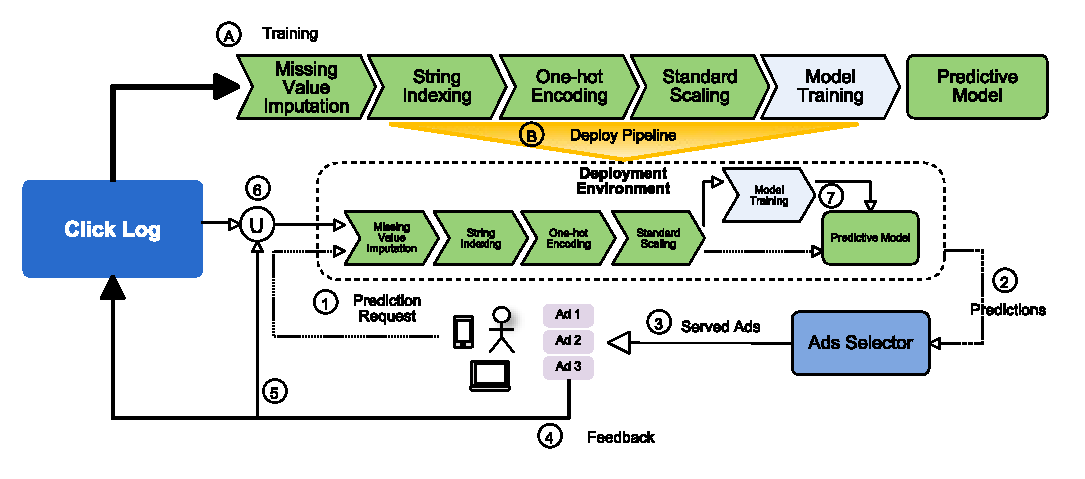
\includegraphics[width=\columnwidth]{../images/improved-example.pdf}
\caption{Ads Serving Continuous Training}
\label{fig:improved-example}
\end{figure}


\section{System Architecture} \label{sec:system-architecutre}
\todo[inline]{explain the statistics collection unit and the scheduler (in more detail)}
The proposed system comprises three main components; model manager, data manager and scheduler, and an independent SGD run-time. 
Figure \ref{fig:system-architecture} gives an overview of the architecture of our system and the interactions among its components.
The data manager first stores the incoming training observations in a buffer and then passes them on to the model manager.
The model manager incrementally updates the model using the training observations.
The model manager is also responsible for receiving prediction requests.
Once it receives a request, it uses the latest version of the model to make a prediction and returns the result to the user.
Both the scheduler and the data manager components are constantly communicating with each other and with the model manager, to obtain the latest statistics, such as the model quality and buffer size.
This in turn helps us to tune the scheduling and sampling rate for future iterations of SGD. 
Next, we explain each component of the system in more detail.


\begin{figure}[t]
\centering
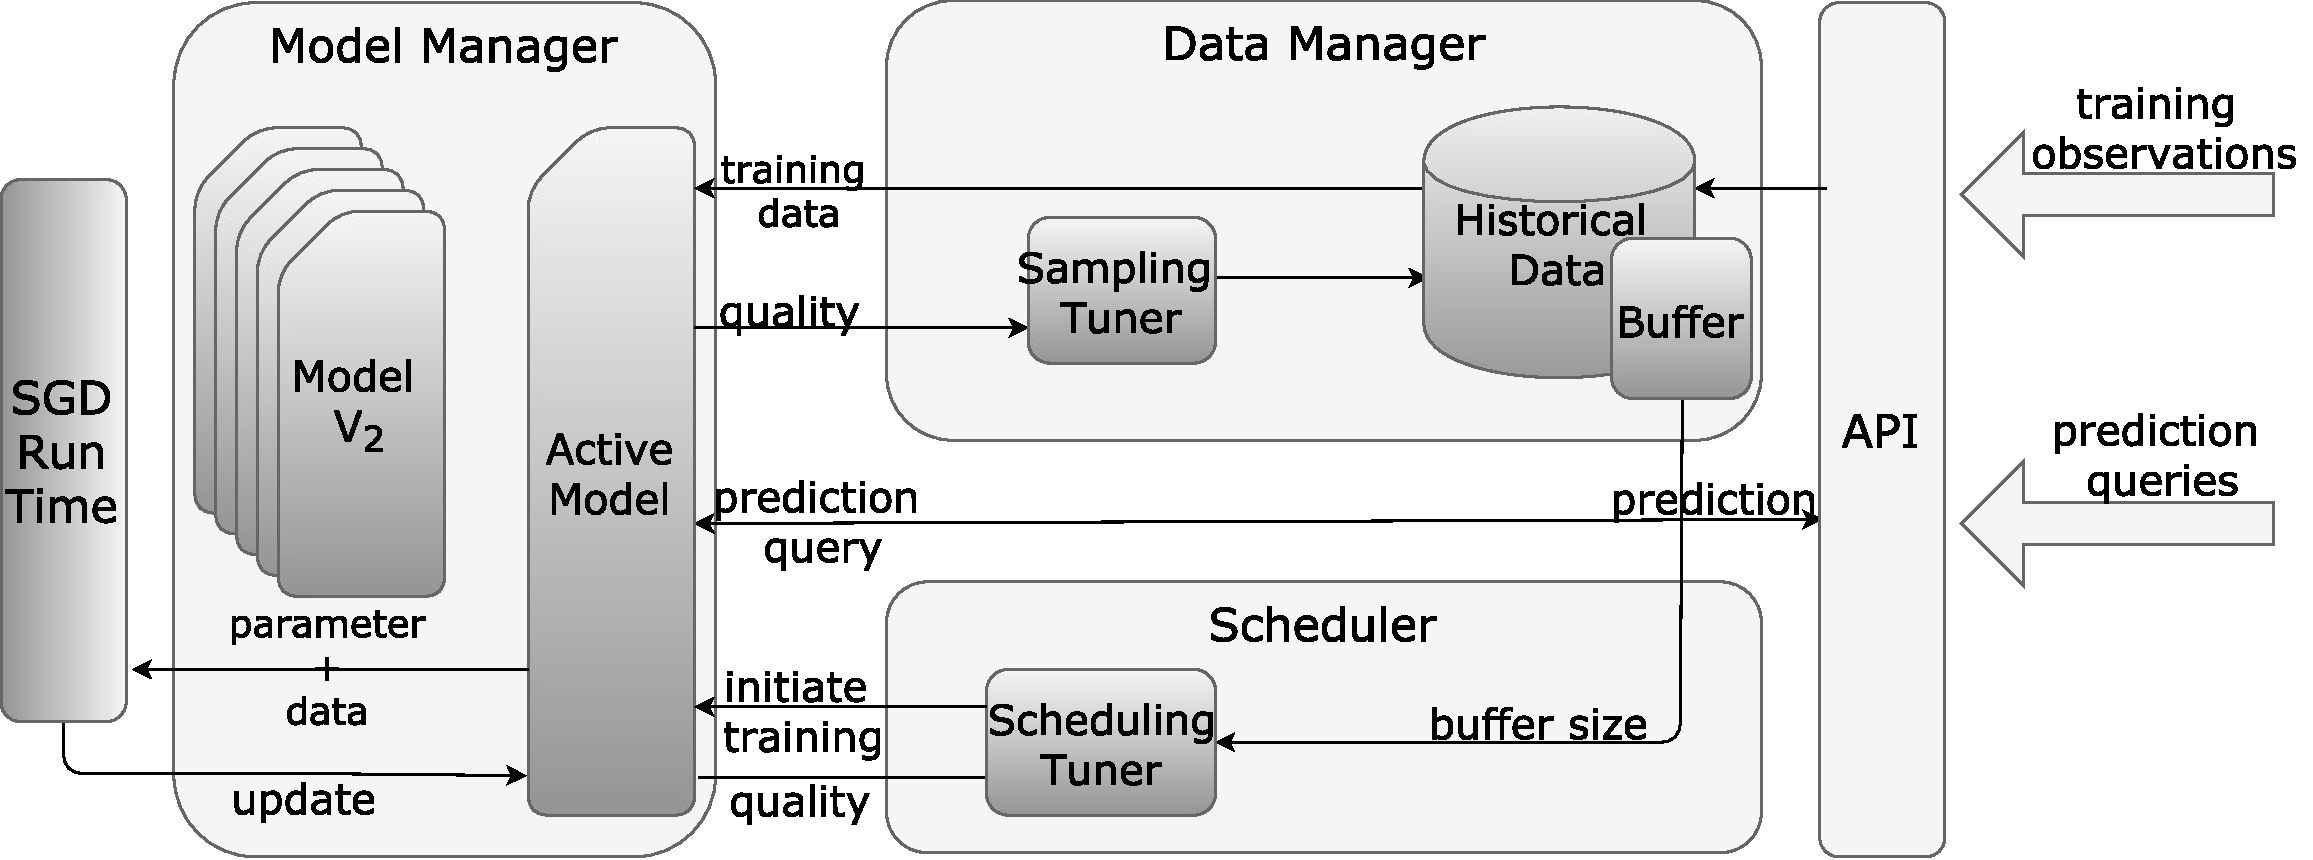
\includegraphics[width=\columnwidth]{../images/system-architecture-final.pdf}
\caption{System Architecture}
\label{fig:system-architecture}
\end{figure}


\subsection{Scheduler}\label{scheduler}
The scheduler component is responsible for scheduling new iterations of SGD.
Intuitively, the best time to execute an iteration is when the system is not under heavy load.
A new iteration of SGD is also executed when the system receives more training data than can be handled by the intermediate buffer.
If the model is not updated with the new training items frequently, the quality decreases.
This decrease in the quality is more rapid if the distribution of the data is changing.
In our prototype, the scheduling rate is controlled by a user defined parameter, \textit{max\_buffer\_size}.
When the intermediate buffer's size reaches \textit{max\_buffer\_size}, the scheduler executes a new iteration of SGD.
It is important to note that the scheduling rate affects the quality of the model.
In Section \ref{evaluation}, we investigate the effect of scheduling rate on model quality.
If no new training data is available, the model parameters will eventually converge and any further training iterations will not have any effect on the model quality.
\todo[inline]{R3: How is the convergence detected?}
Therefore, the scheduler component has to communicate with the model manager in order to detect whether the model parameters have converged and stop further iterations until more training data becomes available.

\subsection{Data Manager} \label{data-manager}
In order to execute an iteration of SGD, we need to combine the training data that arrives at the system in real-time with the data stored on disk.
The data manager is responsible for storing the incoming training observations in an intermediate buffer.
Upon a new training iteration, the data manager accesses the historical data stored on disk and provides a sample.

Different sampling strategies can be used to provide the sample.
In our current prototype, the data manager uses a simple unified random sampling method to generate this sample.
More advanced methods, such as Reservoir \cite{vitter1985random} or weighted random sampling can also be used to generate the sample.
Reservoir sampling is typically used to generate samples from large datasets that do not fit in memory, whereas weighted random sampling is used when data elements have different weights.
In an online machine learning scenario, recent items are more important for training the model and are assigned a bigger weight than older items.
Therefore, weighted random sampling can generate samples that can contribute to the training of a better model.

The data from the sample and the data in the buffer are merged to create the dataset for next training iteration.
The data manager provides access to this dataset for the model manager in order to further train the model.
The data manager also communicates with the scheduler in order to inform it when the intermediate buffer is becoming full and a new training iteration is required. 

The created data set consists of the data inside the buffer and a sample of the historical data as described earlier.
The sampling rate is a system parameter that has to be configured.
It can be pre-configured to a constant value based on the application.
However, using the feedback from the system's model manager (Section \ref{model-manager}), the sampling rate can be adjusted.
For example, when the data distribution is changing, a smaller sampling rate places more emphasis on the data that arrived recently. 
This is similar to the problem of concept drift where the distribution of the incoming data changes overtime.
This renders historical data less important and as a result a smaller sample of the historical data (or none at all) will give more importance to the data in the buffer and help the model to adopt faster to the concept drift.
However, if there is no concept drift in the data, a larger sampling rate will increase the quality of the model after a training iteration.
Another effect that the sampling rate has on the system is the training iteration running time.
A larger sampling rate increases the running time of each training iteration as more data has to be processed.
In Section \ref{evaluation}, we investigate the effects of different sampling rates on both the quality and performance of the system.

Moreover,  new data sets can be registered in data manager.
In our current prototype, new data sets first have to be stored on disk, and data manager can be informed of the data path.
Newly available data sets are used in the subsequent SGD iterations.

\todo[inline]{R2: The difference of incremental update and SGD update needs clarification. In the experiment, they are used in different approaches (baseline+ is using incremental update and Continuous is using SGD). But, the second sentence of the last paragraph of sec 5.3 says both updates are applied in Continuous. BD: I have used incremental to refer to online learning. Whereas in some literature incremental may also refer to mini batch updates. I think the reviewers comment is already addressed in section \ref{subsec:setup}}
\subsection{Model Manager} \label{model-manager} 
An important part of the system is the model manager component.
It is responsible for storing the model, answering prediction queries, and performing incremental and batch updates to the model.
Listing \ref{model-manager-api} shows the API of the model manager.
The API is used to interact with other components as well as end-users of the system.
The scheduler component uses \textit{update} and \textit{update\_iteration} to instruct the model manager to perform incremental or batch updates (one iteration of SGD) to the model.
Upon a new prediction query, the \textit{predict} method is called to provide the end-user with the label of the given input.

\noindent\begin{minipage}[t]{\linewidth}
\begin{lstlisting}[language=java, basicstyle=\small\ttfamily, frame=tb ,columns=fullflexible,
showstringspaces=false,label=model-manager-api,caption=Model Manager API, numberstyle=\tiny]
def update(x,y)

def update_iteration(X,Y)

def predict(x): Label

def error_rate(X_test, Y_test): Double

\end{lstlisting}
\end{minipage}


The \textit{error\_rate} method returns the error rate of the model using the provided test dataset.
As described earlier, constant monitoring of the quality is required in order to adjust the scheduling and sampling rate.
When the error rate is stagnating, the model has converged using the existing data.
Therefore the model manager informs scheduler not to schedule any new iterations until new training observations have arrived at the system.
\todo[inline]{R3: How is this done exactly?}
Similarly as explained in Section \ref{data-manager}, an increase in the error rate may indicate a change in distribution of the data.
As a result, reducing the sampling rate will place more emphasis on recent data (in the intermediate buffer) and help adapt the model to the changes in the distribution.

The model manager also keeps track of the changes that are made to the model.
The model is updated both through incremental learning and SGD-iteration.
The model manager creates snapshots of the model in two different scenarios; after a series of incremental updates are made and after each training iteration.
\todo[inline]{R3: What is the algorithm here?}
This versioning of the models is essential.
When there is a rapid change in the distribution of the incoming data (a sudden concept drift) or when there are anomalies in the data, it is sometimes necessary to revert back to a version before the change in distribution occurred.
In case of concept drift, new training iterations should be scheduled that only use the data in the buffer.
Moreover, in case of anomalies in the data, they have to be identified and discarded before any further model updates could happen.

\subsection{SGD Run-Time} 
All components of our model serving system described so far are not limited to any specific run-time.
We have decoupled the components from the actual run time of the system.
Any system capable of performing incremental and batch SGD updates efficiently are suitable options for our system.
Apache Flink \cite{carbone2015apache} and Apache Spark \cite{zaharia2010spark} are distributed data processing platforms that work with data in memory and have support for iterative algorithms, which makes both of them ideal options for our SGD run-time.
In our current prototype, we are using Apache Spark \cite{zaharia2010spark} as our SGD run-time.

The model manager is the component responsible for communicating with the SGD run-time.
In the current version of our prototype, the model manager requests Spark to perform both incremental and batch updates to the model.
Both types of updates are supported by the built in machine learning library of Spark.
The choice of run-time for SGD slightly influences the data manager as well.
In our prototype, historical data is stored on the Hadoop Distributed File System (HDFS) \cite{shvachko2010hadoop}.

\todo[inline]{R3: The paper has a point that not only the resource consumption is reduced by incremental update, but also the prediction accuracy can be improved due to adapting the model to newly seen data. The system uses a sampling component to use a subset of historical data in each SGD update. However, a non-incremental retraining can also achieve the same adaptation by weighing towards the newly seen data (e.g., learning with concept drifting). Therefore, the ideas of incremental update and adaptation to concept drift should not be confused. The evaluation in this paper does not clearly decouple them. BD: Interesting insight. We have to address this.}